\paragraph{\trHamiltonian\trIsotopy。}\label{sub:hamiltonian-isotopies}
我们的下一个话题是\trContinuationMap{}的一种高阶推广，取\cref{sub:moving-boundary-conditions}
中的意义。我们只给出一个简略的概览，略去技术性的方面。
我们将在上文引入的 \trAinfty-\trCategory{} $\scr{F}(M)^{\mathrm{pr,free}}$ 中工作。设
$(\phi^s)$（$0\le s\le 1$）是 $G=\mathrm{Aut}(M,\partial M)$ 中的一条\trIsotopy，%
从 $\phi^0=\mathrm{Id}$ 走到 $\phi^1=\phi$。仿照
\eqref{eq:isotopy-characteristic-element} 的构造，可以对每个 $(L,\gamma)$ 联系一条上链
\begin{equation*}
T^0\in CF^{\mathrm{pr}}\bigl((L,\gamma),\phi(L,\gamma)\bigr)
\end{equation*}
这指的是：取\trUpperHalfPlane{} $H$，配以由\trIsotopy{} $\phi^s(L)$ 给出的移动\trLagrange\trBoundaryCondition，%
并配备一个与给定\trFloerDatum{}\trCompatible{}的\trPerturbationDatum。注意，%
\trPerturbationDatum{}的选取必然破坏 $H$ 的\trHolomorphic\trAutomorphism{}群。因此，更自然的想法%
或许是：把 $H$ 看成一个在内部带有附加\trMarkedPoint{}（比如说 $z=i$）的\trSurface，%
用它来\trStabilization{}。
沿着这一提示，我们更一般地考虑一个 $(d{+}1)$ \trPointedDisc{} $S$，带有附加的内部%
\trMarkedPoint{} $z$ 与一组\trStriplikeEnd，以及一组\trObject{} $(L_k,\gamma_k)$
（$k=0,\ldots,d$）。取 $0=s_0\le s_1\le\cdots\le s_{d+1}=1$，并在 $S$ 上配备移动%
\trBoundaryCondition：在每段 $C_k$（$0\le k\le d$）上，从 $\phi^{s_k}(L_k)$
走到 $\phi^{s_{k+1}}(L_k)$。做完这些之后，在 $S$ 上选取一个\trPerturbationDatum，%
使其在入端与出端\trStriplikeEnd{}上的行为分别由对子
$((L_0,\gamma_0),\phi(L_d,\gamma_d))$ 与
$(\phi^{s_k}(L_{k-1},\gamma_{k-1}),\phi^{s_k}(L_k,\gamma_k))$ 的\trFloerDatum{}
确定。注意，按 $\scr{F}(M)^{\mathrm{pr,free}}$ 的定义，后者经由 $\phi^{s_k}$
从对子 $((L_{k-1},\gamma_{k-1}),(L_k,\gamma_k))$ 的\trFloerDatum{}诱导而来。我们希望%
这一切都\trSmooth{}地依赖于\trComplexStructure{}与\trMarkedPoint{}的选取，这意味着%
我们看的不是单个 $(S,z)$，而是所有带一个附加内部\trMarkedPoint{}的 $(d{+}1)$
\trPointedDisc{}的\trModuliSpace{} $\scr{R}^{d+1,1}$ 及其上方的\trUniversal\trFamily。%
这个空间有一个 Deligne--Mumford 型的\trCompactification
\begin{equation}\label{eq:moduli-with-interior-point}
\bar{\scr{R}}^{d+1,1}=\coprod_{(T,v_\star)}
\Bigl(\scr{R}^{|v_\star|,1}\times\prod_{v\neq v_\star}\scr{R}^{|v|}\Bigr)
\end{equation}
其\trStratum{}由带一个取定\trVertex{} $v_\star$ 的 $d$ \trLeafedTree{}标引（$v_\star$ 的%
\trValency{}可以是任意正数，而其余\trVertex{}应至少三价）。
诸\trStriplikeEnd{}、诸 $s_k$ 以及\trPerturbationDatum{}的选取，还须满足一个相对于
\eqref{eq:moduli-with-interior-point} 的适当\trConsistency{}条件；我们不把它显式地%
表述出来。于是便可以考察相关的\trModuliSpace{}：由对子
$(r\in\scr{R}^{d+1,1},\ u\colon\scr{S}^{d+1,1}_r\to M)$ 组成，其中 $u$ 是一个%
\trInhomogeneous\trPseudoholomorphicMap。在该空间中计数具有适当\trAsymptotic{}行为的点，就定义了映射
\begin{equation*}
\begin{split}
T^d\colon CF^{\mathrm{pr}}\bigl((L_{d-1},\gamma_{d-1}),(L_d,\gamma_d)\bigr)\otimes\cdots\\
\cdots\otimes CF^{\mathrm{pr}}\bigl((L_0,\gamma_0),(L_1,\gamma_1)\bigr)
&\longrightarrow CF^{\mathrm{pr}}\bigl((L_0,\gamma_0),\phi(L_d,\gamma_d)\bigr).
\end{split}
\end{equation*}
这里，我们又一次用到了
$CF^{\mathrm{pr}}(\phi^{s_k}(L_{k-1},\gamma_{k-1}),\phi^{s_k}(L_k,\gamma_k))$
可以\trCanonical{}地等同于
$CF^{\mathrm{pr}}((L_{k-1},\gamma_{k-1}),(L_k,\gamma_k))$ 这一事实。诸 $T^d$ 满足方程
\begin{equation}\label{eq:hamiltonian-isotopy-aoo}
\begin{split}
\sum_{m,n}\mu^{d-m+1}_\star\bigl(\phi_\star^1(a_d),\ldots,\phi_\star^1(a_{n+m+1}),%
T^m(a_{n+m},\ldots,a_{n+1}),a_n,\ldots,a_1\bigr)\\
+\sum_{m,n}T^{d-m+1}\bigl(a_d,\ldots,a_{n+m+1},\mu^m(a_{n+m},\ldots,a_{n+1}),a_n,\ldots,a_1\bigr)=0
\end{split}
\end{equation}
（图 10.1 展示了两类被加项所对应的\trDegenerate，并同时标出移动的与不移动的%
\trBoundaryCondition）。由于\trAFunctor{} $\phi_\star$ 的高阶项为零，而我们眼下%
又无须操心正负号，\eqref{eq:hamiltonian-isotopy-aoo} 恰好就是 $T$ 成为由恒同到
$\phi_\star$ 的\trNaturalTransformation{}的条件。正如\cref{sub:moving-boundary-conditions}
末尾已经指出的，每个 $T^0$ 在 $H\scr{F}(M)^{\mathrm{pr,free}}$ 中是一个\trIsomorphism，%
故由\cref{thm:right-composition-iso}，$T$ 在 \trAFunctor{}的\trCohomology\trCategory{}%
中是一个\trIsomorphism。把这一结果\trTransfer{}到\trQuasiequivalence{}的%
\trAinfty-\trCategory{} $\scr{F}(M)^{\mathrm{pr}}$ 上，我们便有：
\begin{proposition}\label{thm:hamiltonian-isotopy-iso}
设 $\phi\in\mathrm{Aut}(M,\partial M)$ 是一个与恒同\trIsotopy{}的\trAutomorphism。%
那么由 $\phi$ 诱导的\trAFunctor{}在
$H(\mathit{fun}(\scr{F}(M)^{\mathrm{pr}},\scr{F}(M)^{\mathrm{pr}}))$ 中与恒同\trFunctor{}%
\trIsomorphic。\noqed
\end{proposition}
换句话说，$\mathrm{Aut}(M,\partial M)$ 在 $\scr{F}(M)^{\mathrm{pr}}$ 上的\trCoherent{}%
作用下降为 $\pi_0(\mathrm{Aut}(M,\partial M))$ 的一个弱作用。
\begin{remark}\label{thm:group-cohomology-obstruction}
取一个群 $\varGamma$ 作用在\trCategory{} $A$ 上的弱作用这一一般设置。令
$HH^0(A,A)^\times$ 为从 $\mathrm{Id}_{A}$ 到其自身的%
\trFunctor\trIsomorphism{}构成的集合，并经\trComposition{}使之成为一个\trAbelianGroup。%
使该作用变得\trCoherent{}的\trObstruction{}是一个群\trCohomology{}类，更确切地说，是
$H^2(\varGamma;HH^0(A,A)^\times)$ 中的一个元素。现在设
$\varGamma=\pi_0(G)$、$G=\mathrm{Aut}(M,\partial M)$，并且为简单起见取
$A=H\scr{F}(M)^{\mathrm{pr}}$ 为\trDonaldson--\trFukayaCategory。在这种情形，%
\trObstruction{}类承自 $H^2(\pi_0(G);\pi_1(G))$ 中的一个\trCanonical{}类（它对任何\trTopologicalGroup{}都存在），%
经由一个用 [123]、[1] 的方法定义的\trHomomorphism{} $\pi_1(G)\to HH^0(A,A)^\times$。%
在 \trAinfty-\trCategory{}的层面上大概也有一个平行的陈述，但我们未曾探究其细节。%
无论如何，即便如此，这也仍然只是故事的一部分。正如\cref{thm:converse-construction-remark}
中那样，我们对 \trAinfty-\trCategory{}之\trCoherent{}群作用的定义应当被看作一个%
初步的近似；人们可以期待，最终的概念会涉及 $G$ 的整个\trHomotopy{}型，而不仅仅是\trDegree
$\le 1$ 的那些\trHomotopy{}群。
\begin{figure}
\centering
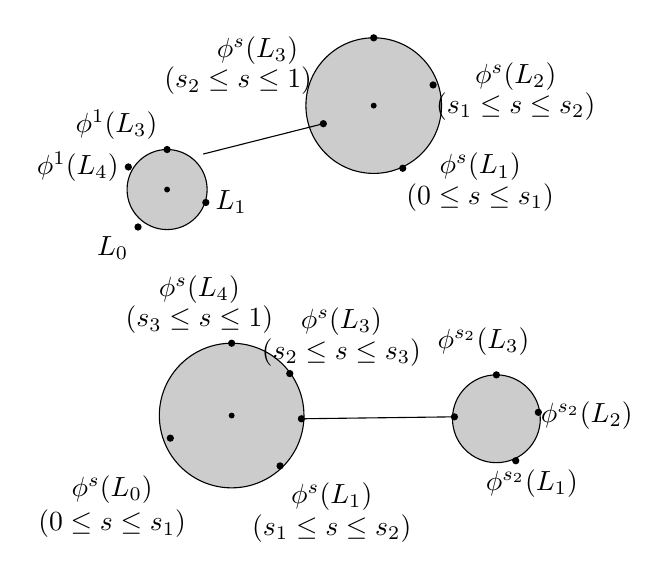
\begin{tikzpicture}[scale=0.82]
\begin{scope}[shift={(0,3.2)}]
\draw[fill=black!20] (4.4,1.3) circle (1.05);
\fill (4.4,1.3) circle (1.3pt);
\draw[fill=black!20] (1.2,0) circle (0.62);
\fill (1.2,0) circle (1.3pt);
\fill (1.2,0.62) circle (1.6pt) node[above left] {$\phi^1(L_3)$};
\fill (0.6,0.35) circle (1.6pt) node[left] {$\phi^1(L_4)$};
\fill (1.8,-0.2) circle (1.6pt) node[right] {$L_1$};
\fill (0.75,-0.58) circle (1.6pt) node[below left] {$L_0$};
\draw (1.76,0.55) -- (3.62,1.02);
\fill (3.62,1.02) circle (1.6pt);
\fill (4.4,2.35) circle (1.6pt);
\fill (5.32,1.62) circle (1.6pt);
\fill (4.85,0.33) circle (1.6pt);
\node at (2.6,2.15) {$\phi^s(L_3)$};
\node at (2.3,1.68) {$(s_2\le s\le 1)$};
\node at (6.6,1.75) {$\phi^s(L_2)$};
\node at (6.6,1.28) {$(s_1\le s\le s_2)$};
\node at (6.05,0.35) {$\phi^s(L_1)$};
\node at (6.05,-0.12) {$(0\le s\le s_1)$};
\end{scope}
\begin{scope}[shift={(0,-1.2)}]
\draw[fill=black!20] (2.2,0.9) circle (1.12);
\draw[fill=black!20] (6.3,0.85) circle (0.68);
\fill (2.2,2.02) circle (1.6pt);
\fill (3.1,1.55) circle (1.6pt);
\fill (3.28,0.85) circle (1.6pt);
\fill (2.95,0.12) circle (1.6pt);
\fill (1.25,0.55) circle (1.6pt);
\fill (2.2,0.9) circle (1.3pt);
\fill (6.3,1.53) circle (1.6pt);
\fill (6.95,0.95) circle (1.6pt);
\fill (6.6,0.2) circle (1.6pt);
\draw (3.28,0.85) -- (5.65,0.88);
\fill (5.65,0.88) circle (1.6pt);
\node at (1.7,2.85) {$\phi^s(L_4)$};
\node at (1.7,2.38) {$(s_3\le s\le 1)$};
\node at (3.9,2.35) {$\phi^s(L_3)$};
\node at (3.9,1.88) {$(s_2\le s\le s_3)$};
\node at (3.75,-0.35) {$\phi^s(L_1)$};
\node at (3.75,-0.85) {$(s_1\le s\le s_2)$};
\node at (0.35,-0.25) {$\phi^s(L_0)$};
\node at (0.35,-0.78) {$(0\le s\le s_1)$};
\node at (6.1,2.05) {$\phi^{s_2}(L_3)$};
\node at (7.7,0.9) {$\phi^{s_2}(L_2)$};
\node at (6.85,-0.15) {$\phi^{s_2}(L_1)$};
\end{scope}
\end{tikzpicture}
\caption{}\label{fig:hamiltonian-isotopy-degenerations}
\end{figure}
\end{remark}
